%!TEX root = ../main.tex
\chapter{Materiales y Métodos}
\label{chap:MaterialesYMetodos}

En este capítulo se mostrarán los recursos necesarios y los pasos seguidos para llegar a los objetivos propuestos en este trabajo. Se describen a lo largo de este capítulo; La principal fuente de datos utilizada (DNCP \cite{DatosAbiDNCP:online}, ver sección \ref{section:portalDNCP}) y el principal recurso no ontológico utilizado (OCDS, ver sección \ref{section:OCDS}) para el desarrollo de la ontología. Así también una breve reseña del proceso de desarrollo de la ontología (ver sección \ref{section:desarrolloOntologia}), luego explicamos el proceso de despliegue y análisis de los resultados (ver sección \ref{section:despliegue}).

\section{Portal de Datos Abiertos de la DNCP}
\label{section:portalDNCP}

En Paraguay, la DNCP \cite{DatosAbiDNCP:online}, organismo del estado que publica datos de los procesos de contrataciones, posee un portal de datos abiertos donde publica datos en tiempo real de los estados de las licitaciones públicas del país. 

Esta plataforma es fundamental para este y otros trabajos de investigación basados en datos de contrataciones ya que posee los datos de prueba y el escenario de caso de uso. En el proceso se realizaron reuniones e intercambios de correos electrónicos tanto con el equipo técnico encargado de mantener el portal, como el equipo legal de la dirección a fin de conocer el contexto, las funcionalidad, las limitantes y las necesidades de la institución. De no tener este contacto directo, el objetivo de este trabajo pudo haber sido comprometido.

La plataforma posee las siguientes características y funcionalidades principales

\begin{enumerate}
    \item Lista de datos. Con el fin de que los usuarios que necesitan ver, analizar y descargar en formato CSV los datos detallados de todos los registros de contrataciones.
    \item Visualizaciones de datos para usuarios que deseen ver estadísticas e información agregada.
    \item Una API para desarrolladores que permite manipular datos en formato JSON y JSON-LD de manera programática para cualquier otro uso.
    \item Plataforma de Contrataciones Electrónica, destinada a empresas y personas que deseen presentarse o conocer algún proceso de contratación.
\end{enumerate}

Los datos publicados poseen un diccionario y una ontología creada por la DNCP, la cual sirve como contexto para la API desarrollada. Además la DNCP implementó una API siguiendo el estándar OCDS, que posee un esquema de publicación bien definido en JSON Schema.

A continuación hablaremos del estándar utilizado como recurso no ontológico para el desarrollo de la ontología.

\section{Open Contracting Data Standard}
\label{section:OCDS}

El \textit{Open Contracting Data Standard} (OCDS)\footnote{http://standard.open-contracting.org}  es un estándar amigable y flexible para estructurar información de Contrataciones Públicas y es mantenido por la OCP. El estándar describe qué, cuándo y cómo disponibilizar datos y documentos asociados en las diferentes fases del proceso de contratación. El proyecto promueve la divulgación y participación en las contrataciones públicas creando un estándar abierto de datos simple. OCDS posee un esquema de datos detallado de todos los conceptos así como también la estructura de los datos divulgados, dicho esquema esta disponible el sitio web del estándar \cite{OCDSReleaseSchema:online}. Este esquema ayuda a las personas a comprender todos los campos publicados. Además el estándar posee un guía de implementación a modo de facilitar la implementación\footnote{http://standard.open-contracting.org/latest/en/implementation/}.

El estándar ha ganado especial popularidad en los últimos años y fue implementado por más de 15 países \footnote{https://www.open-contracting.org/resources/es-version-1-1-resumen-sobre-actualizacion-del-estandar/} países hasta el año 2017, donde Paraguay es un de ellos. Es por eso que el mismo ha sido elegido como base de conocimiento principal de dominio de contrataciones públicas.

\section{Planteamiento del problema}
\label{section:planteamientoDelProblema}

A partir del escenario visto en el portal de Datos Abiertos de la DNCP y la implementación del OCDS en este portal nace la pregunta de qué manera se puede lograr una mejor interoperabilidad de datos de distintas fuentes a fin de obtener, de manera automática, información valiosa para lograr mayor transparencia y mejor toma de decisiones. Así como lo mostrado en el capítulo anterior, esto se puede lograr aplicando conceptos de la Web Semántica y desarrollando una ontología que permita lograr esta interoperabilidad semántica. 

En la Figura \ref{img:materialesymetodos} se expone el proceso desarrollado para lograr los objetivos propuestos. Se agrupó en tres fases principales que son: investigación, desarrollo y verificación.

En la fase de investigación se procedió al estudio del estado del arte, luego a la identificación de las ontologías del dominio existentes y de las metodologías de desarrollo de ontologías. Por último se realizó un análisis de la fuente de datos de la DNCP.

En la fase de desarrollo se procedió a desarrollar la ontología basada en el OCDS, luego a la extracción de los datos de prueba para su posterior conversión y almacenamiento y por último se procedió a la creación de un punto de consulta SPARQL.

Por último se procedió a la verificación de lo desarrollado formulando preguntas experimentales expresadas en casos de uso de la ontología y el posterior análisis y conclusión del trabajo. En este punto cabe destacar que al proceder a la verificación de las preguntas experimentales se evidenció la necesidad de volver al proceso de desarrollo de la ontología aplicando algunos ajustes y mejoras detectadas introduciendo así un ciclo iterativo en el proceso hasta concluir exitosamente.


En las siguientes secciones se dará una breve reseña acerca del desarrollo de la ontología y el despliegue de los resultados. 

\begin{figure}[ht!]
    \centering
    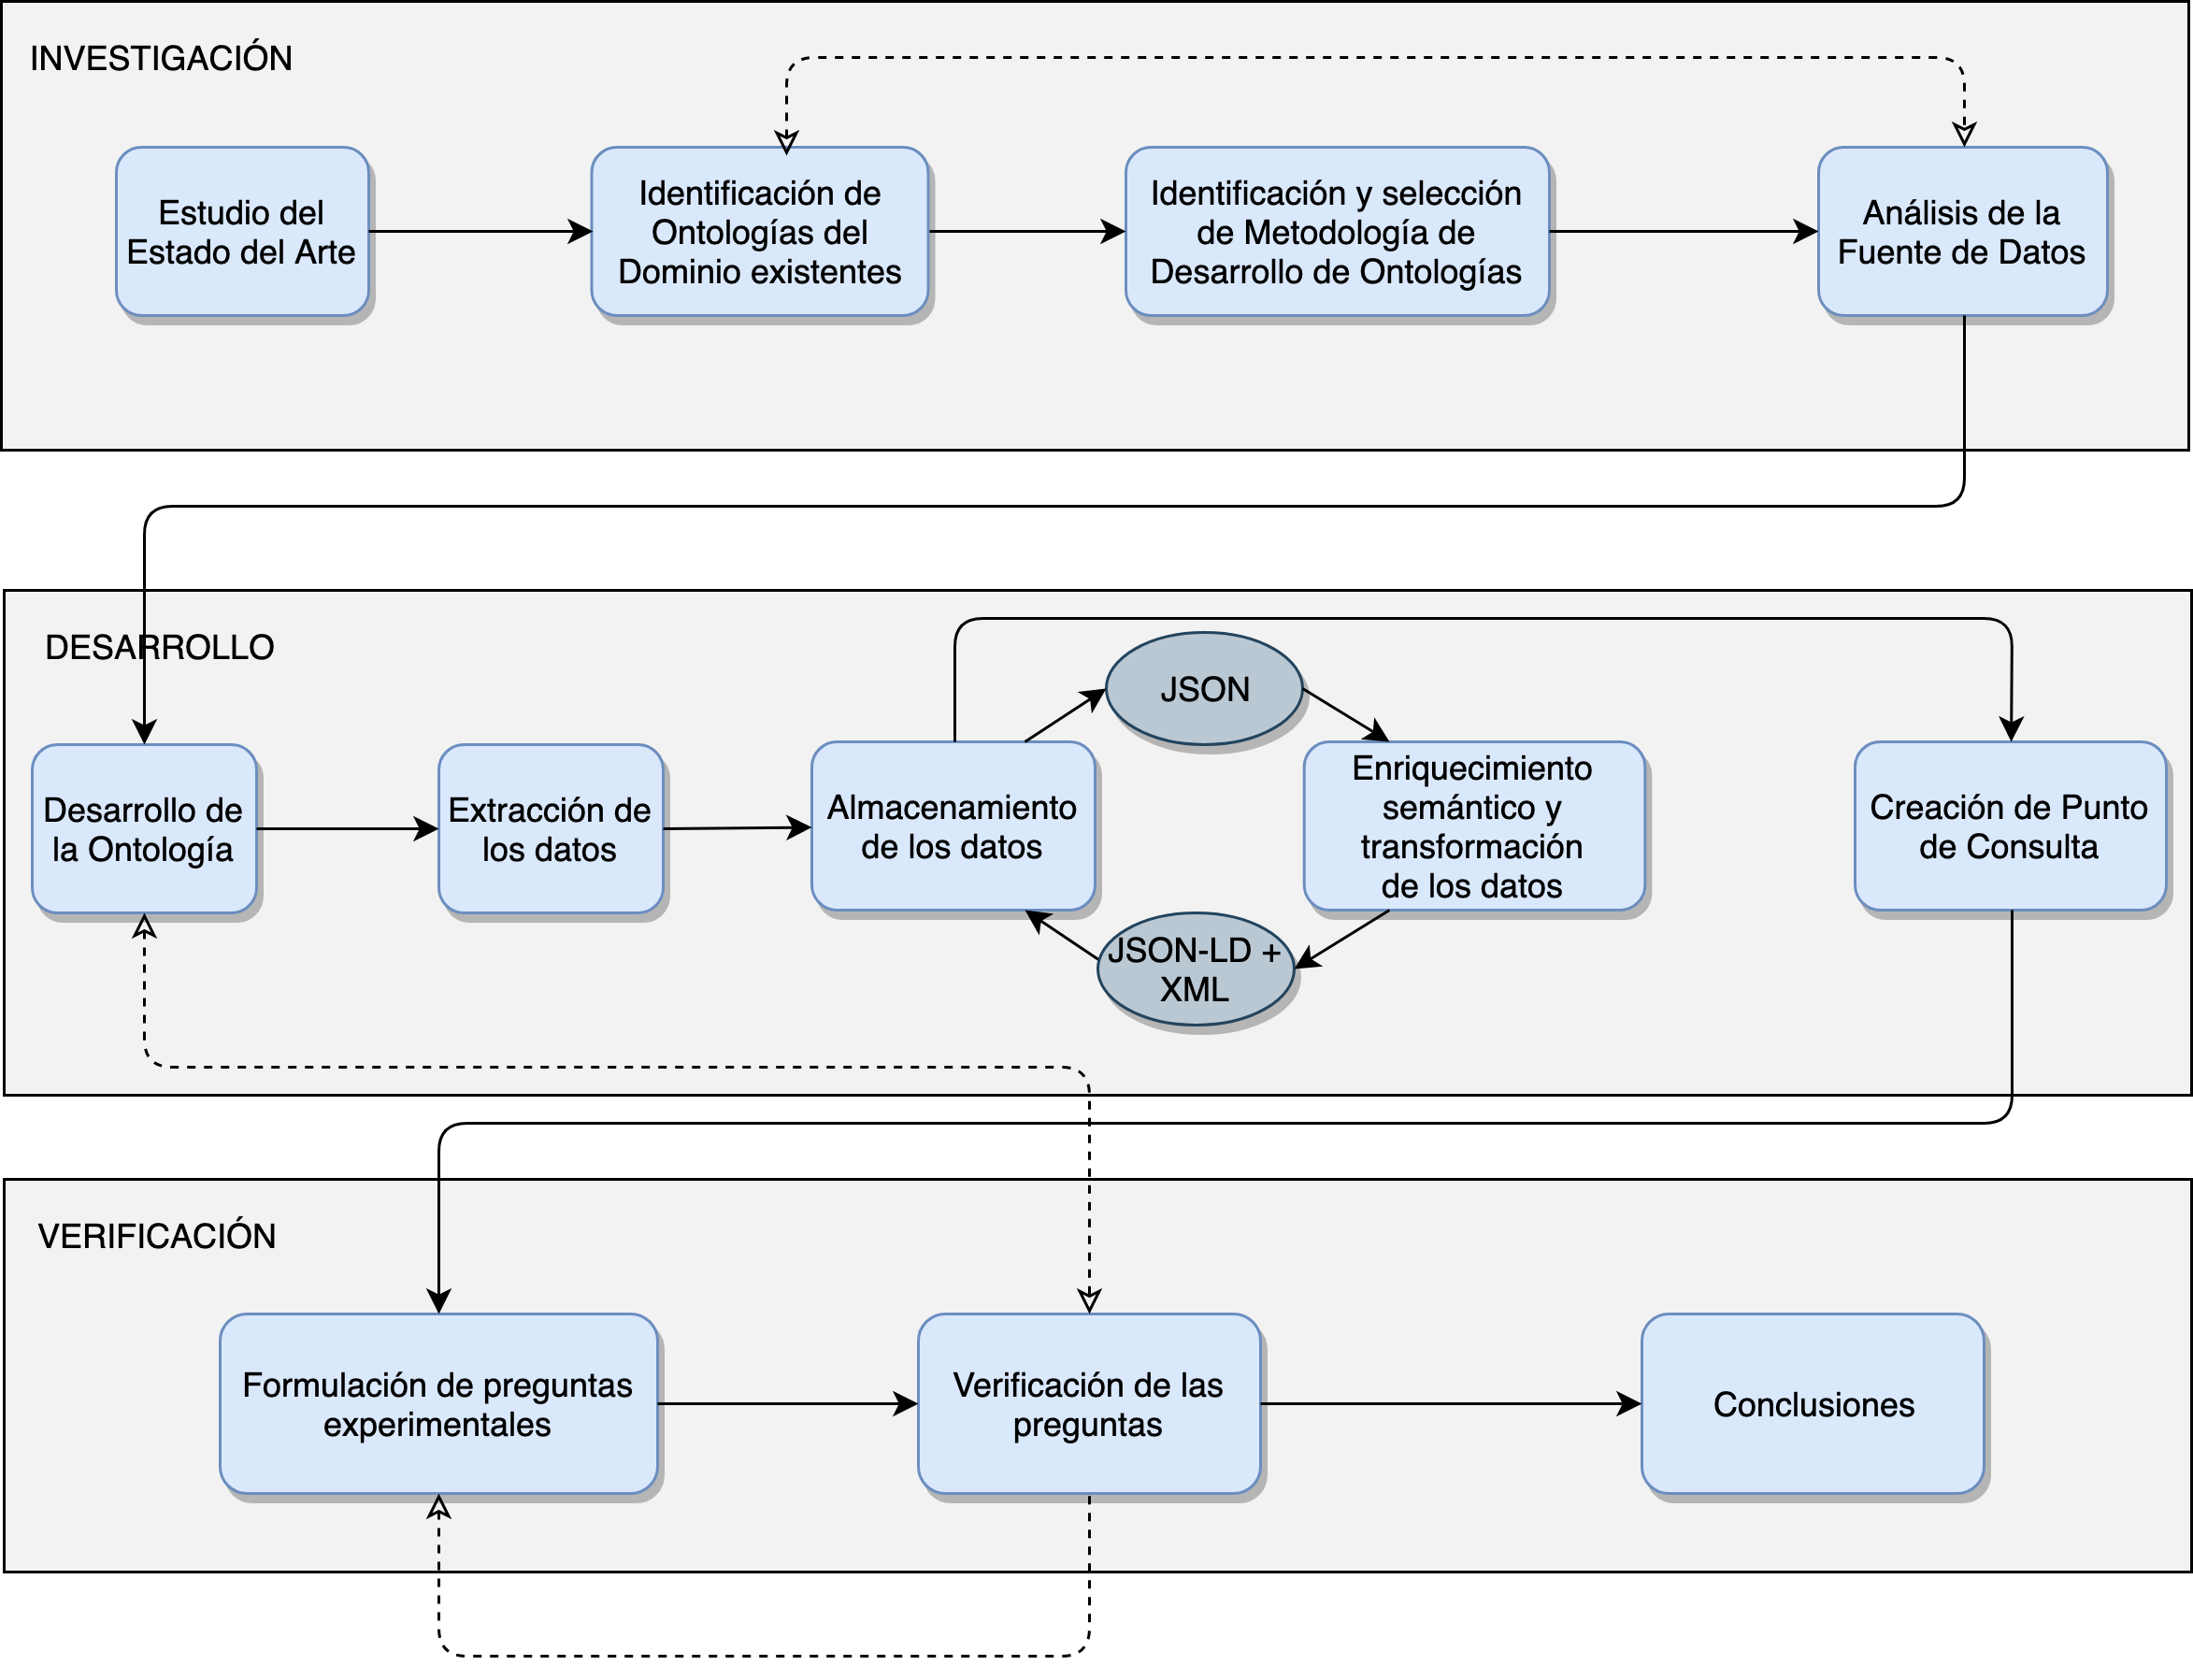
\includegraphics[width=150mm]{figuras/Diagramas-MaterialesYMetrodos.png}
    \caption{Modelo de Ciclo de Vida de desarrollo de la ontología.}
    \label{img:materialesymetodos}
\end{figure}

\section{Desarrollo de la ontología}
\label{section:desarrolloOntologia}

Parte fundamental de este trabajo consiste en el desarrollo de una ontología basada en el estándar de publicación de datos OCDS. Al estándar, como veremos más adelante en este trabajo, se lo clasificó como un recurso no ontológico, ya que formaliza la sintaxis pero describe en lenguaje natural y no en lenguaje formal, la semántica del dominio de conocimiento. 

Se utilizó como guía metodológica de desarrollo de ontología principal NeOn, ya que la misma, según lo que se muestra en la Tabla  \ref{tab:comparacion}, posee mayor especificación en las actividades a desarrollar  y contempla los casos de reuso de recursos ontológicos y no-ontológicos. 

Así como lo anticipa la metodología, el desarrollo de una ontología no es un proceso lineal, a lo largo de todo este trabajo, la misma es alterada y mejorada constantemente para lograr los objetivos propuestos. En el Capítulo \ref{chap:Desarrollo de la Ontologia} se describirá en detalle todo el proceso para llegar al producto final que representa la mayor contribución de este trabajo.

\section{Despliegue y Análisis de Resultados}
\label{section:despliegue}

Para llevar a cabo este trabajo se desarrolló un software de extracción de datos con los cuales se logró demostrar el funcionamiento de la ontología desarrollada, la cual se describirá en el Capítulo \ref{chap:Implementación de la Ontologia}. El proceso consistió en el desarrollo de un software que se encargó de extraer los datos (a ser utilizados en las pruebas) de la plataforma de datos abiertos de la DNCP por medio de la API para desarrolladores. Este software realiza también un proceso de conversión de datos y posterior enlace con la ontología desarrollada. Finalmente, los convierte en formato RDF para luego ser disponibilizados en un Punto SPARQL implementado en un servidor Apache Jena Fuseki. De esta manera fue posible realizar consultas utilizando los datos mencionados y datos de otras fuentes externas.

Con los datos disponibles para la consulta, describimos 5 casos de uso de los datos enriquecidos con la ontología desarrollada que nos ayudan a mostrar que se pueden lograr los objetivos propuestos de este trabajo. Los 5 casos de uso están descriptos en el Capítulo \ref{chap:Contexto experimental}.

%
\section{Especificación de requerimientos de la ontología}

En esta actividad se define el alcance y los requerimientos de la ontología a desarrollar. Como resultado de esta actividad se obtiene el Documento de Especificación de Requerimientos de la Ontología (ORSD). A continuación se detalla el resultado de dicho proceso.
\begin{enumerate}

    \begin{figure}[h!]
        \centering
        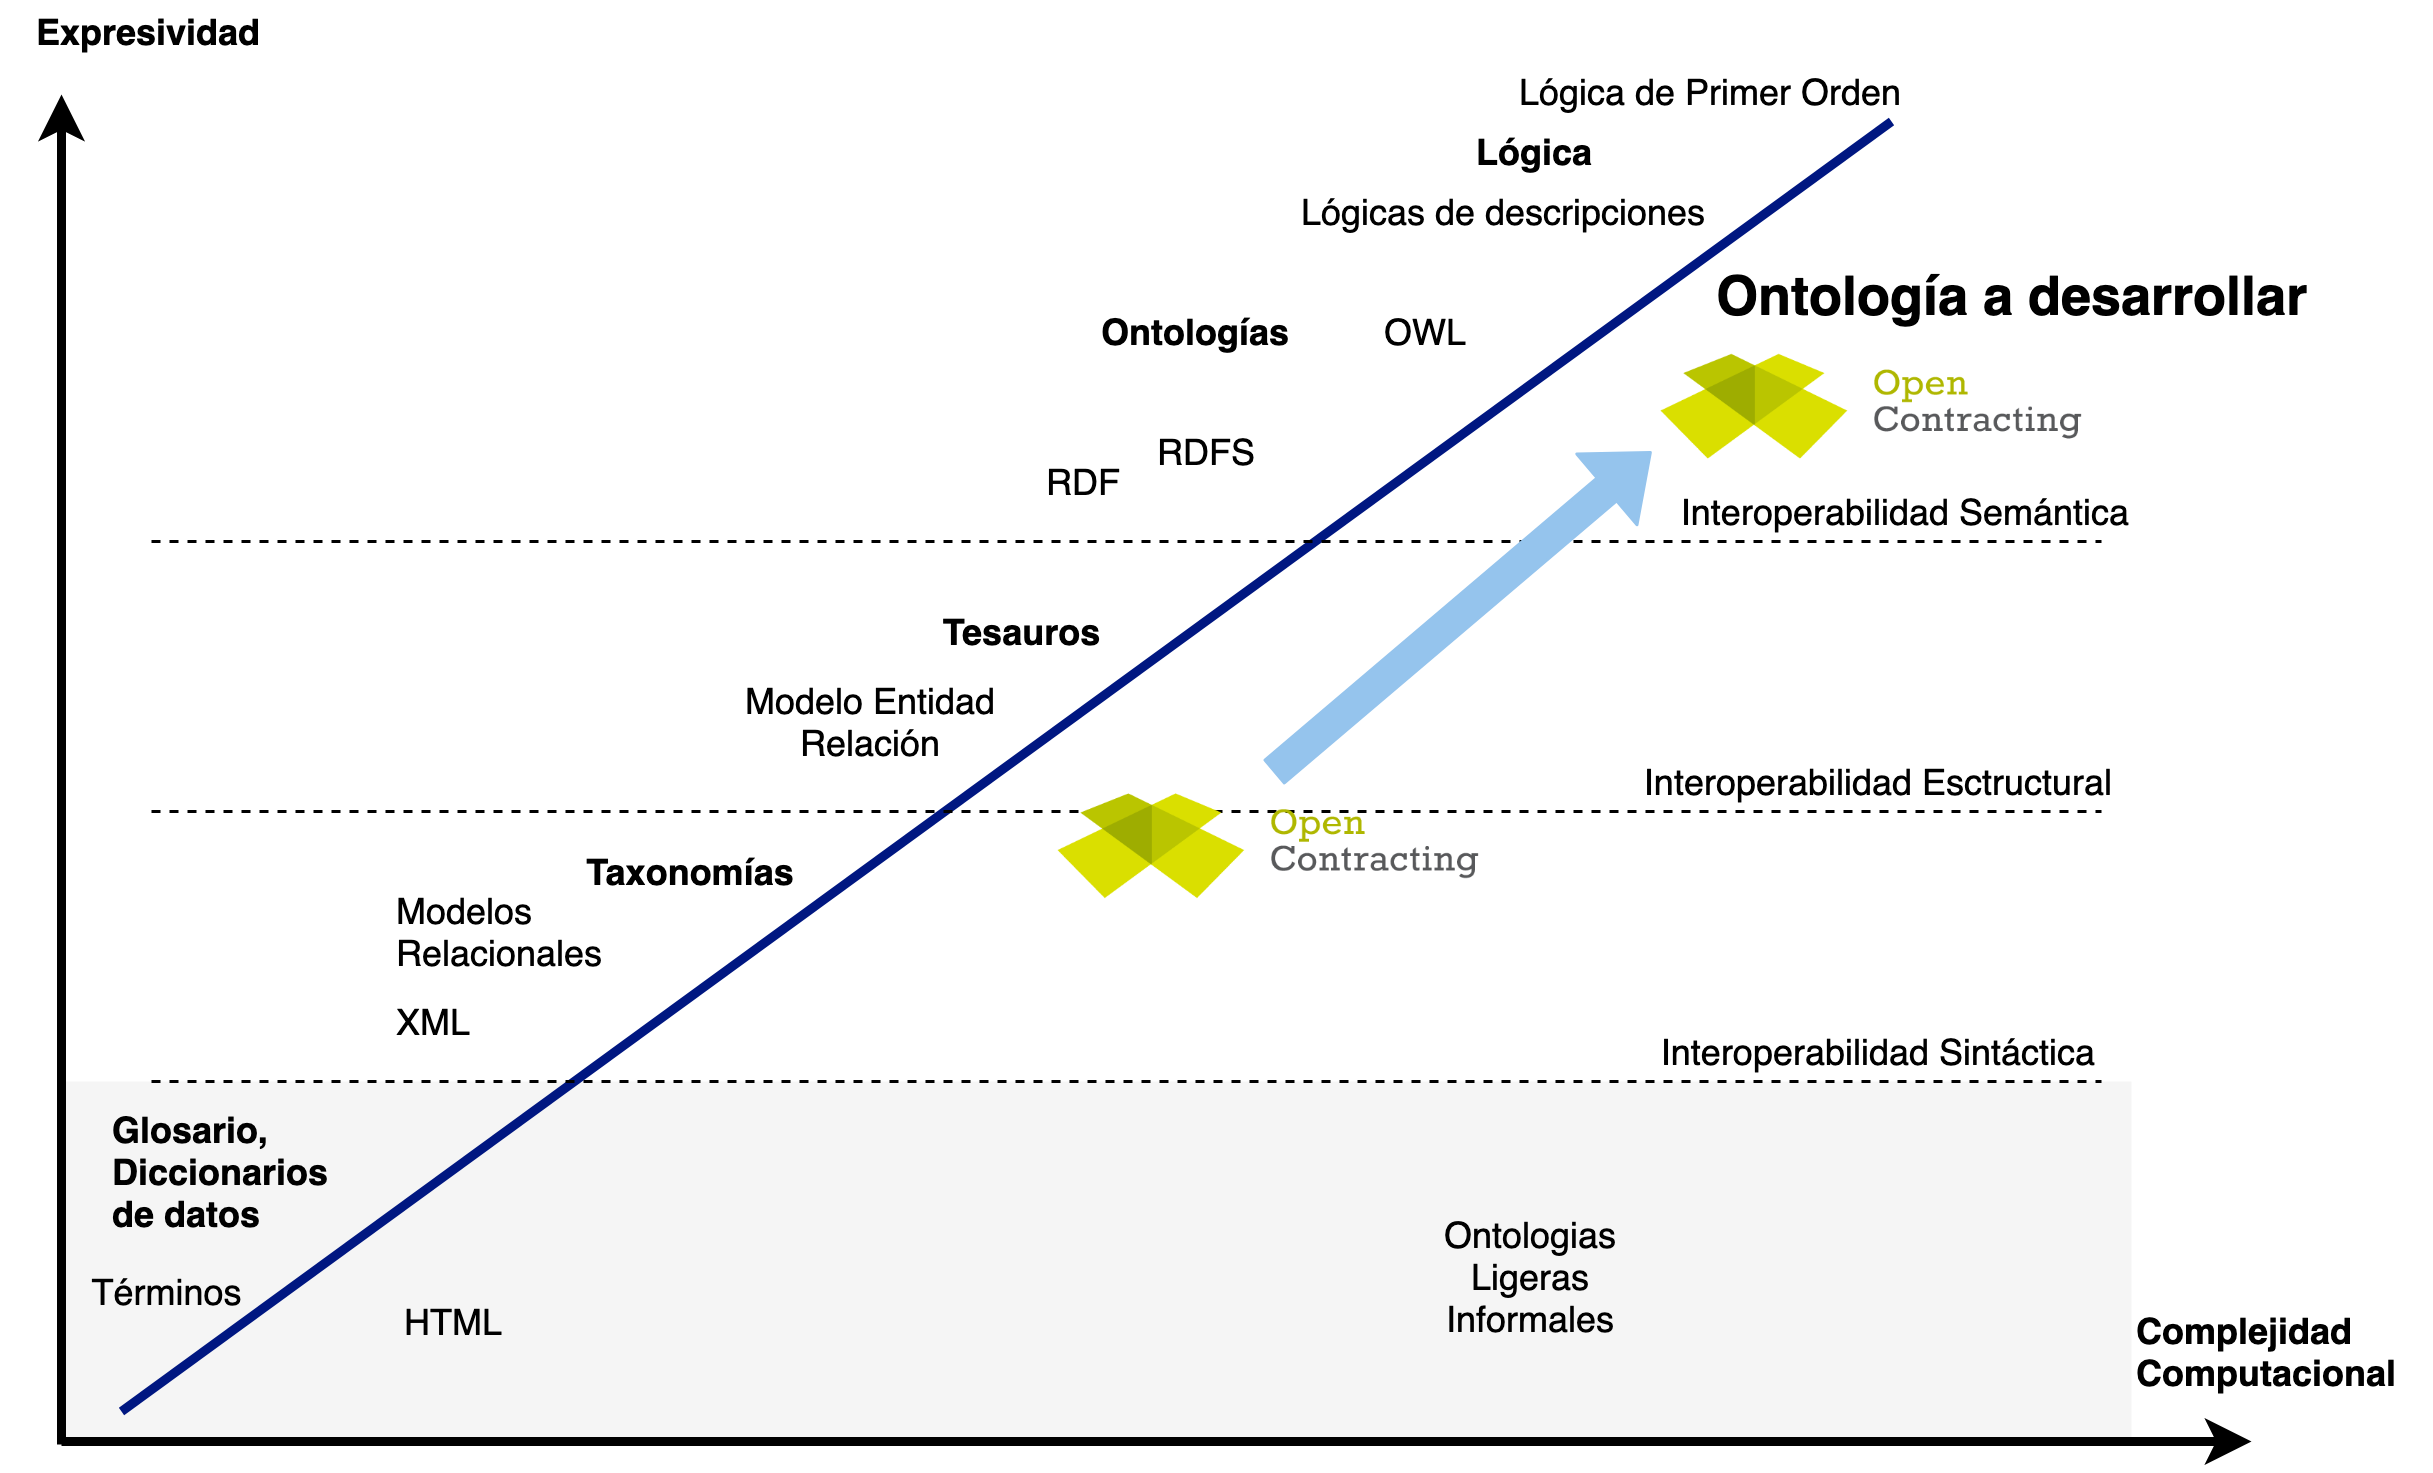
\includegraphics[width=150mm]{figuras/Diagramas-OenContracting.png}
        \caption{Nivel de complejidad semantica de la ontologia a desarrollar}
        \label{img:ocds-ocntology-complejidad}
        \end{figure}
        
\item \textbf{Propósito:} Crear una ontología para el dominio de Contrataciones Públicas para lograr la interoperabilidad semántica con otras fuentes de datos externas utilizando el OCDS como base de conocimiento principal aumentando la formalidad semántica como se muestra en la figura \ref{img:ocds-ocntology-complejidad}


\item \textbf{Alcance:} El alcance de la ontología está delimitada por el vocabulario detallado en la versión 1 del OCDS. Se eligió dicha versión ya en el momento del inicio de esta investigación era la última versión estable del estándar.
\item \textbf{Lenguaje de Implementación.} Se utilizará el lenguaje OWL debido a que es el lenguaje preferido para ontologías en la web semántica recomendado por la W3C \cite{OWLSeman72:online}, y se requiere de una ontología lo suficientemente ligera y explícita que se pueda manejar en la web semántica.
\item \textbf{Grupo Objetivo.}La ontología está orientada a:
\begin{enumerate}
    \item Expertos del dominio de Contrataciones Públicas que quieran realizar consultas ad-hoc sobre datos.
    \item Desarrolladores de software que deseen implementar el OCDS.
    \item Desarrolladores de software que necesiten integrar datos de contrataciones públicas con otras fuentes externas. \end{enumerate}
\item \textbf{Usos de la Ontología. }La ontología se utilizará para crear un esquema de publicación en JSON-LD, esto es debido a que la sintaxis JSON es ampliamente conocida y preferida por los desarrolladores \cite{JSON-37:online}, además el OCDS ya posee un esquema de publicación compatible con esta sintaxis. Los datos utilizados se extraerán del portal de datos abiertos de la DNCP.
\item \textbf{Requerimientos No Funcionales: }
\begin{enumerate}
    \item Se optará, en lo posible, por la reutilización de otras ontologías del dominio de Contrataciones Públicas ampliamente utilizadas.
    \item La ontología desarrollada debe ser procesable dentro de las limitaciones de la web semántica, ósea debe ser una ontología ligera.
    \item Debe soportar múltiples lenguajes: inglés y español inicialmente.
\end{enumerate}
\item \textbf{Requerimientos Funcionales. }
    \begin{enumerate}
        \item Gracias a la ontología se podrán responder las mismas preguntas que se responden a través de los datos publicados en formato de JSON y se podrán responder preguntas de todas las fases del proceso licitatorio.
        \item Debe ser compatible con la versión 1 del OCDS.
        \item Los datos deberán poder ser enriquecidos con otras fuentes de datos provenientes de la DNCP y también fuentes externas como Wikidata o DBpedia.
    \end{enumerate}
\item \textbf{Pre-Glosario de Términos.} El glosario fue extraído del diccionario de datos y de la ontología desarrollada por la DNCP. 
\end{enumerate}



\section{Discusión del Capitulo}

En este capítulo se mostraron los recursos necesarios y los pasos seguidos para la llegar a los objetivos propuestos en este trabajo. Se detalló la importancia de la fuente de datos utilizada, el estándar de datos utilizado como base de conocimiento principal y la herramienta metodológica para el desarrollo de la ontología. Además de la manera en que se pretende mostrar la forma de uso del producto desarrollado.

En el siguiente capítulo comenzaremos con el desarrollo de la ontología utilizando la metodología NeOn.




